\section{Design Goals}
\label{sec:Design_Goals}
% Owner: Johanna
% Reviewed: 
%
Given the current, very limited possibilities to simulate a huge, dynamic online marketplace, we came up with a set of specific design goals and restrictions, that we wanted to fulfill to make the platform and the resulting simulation as realistic, dynamic and reactive as possible: 

\begin{description}

\item\textbf{Reactivity:} Allow pricing algorithms to do fully dynamic price updates and look-ups at any time without being refrained by discrete time intervals to enable truly reactive pricing strategies.

\item\textbf{Realism:} Enforce real-life restrictions present in every big real-life marketplace such as a limited amount of price updates per time interval to avoid advantages by constantly changing prices.

%\item\textbf{Flexibility:} Offer the greatest possible flexibility in terms of scalability and adaptivity of the system to make the system easily expandable and adaptable to new possible design goals or user needs. --> split up into scalability and adaptivity

\item\textbf{Scalability and Adaptability:} The system should be highly scalable and easily expandable to account for all possible demands such as a very high load, the simulation of huge marketplaces or the addition of completely new components and features.    

\item\textbf{Flexibility:} Offer the greatest possible flexibility to make the system adaptable to user needs and new possible design goals. Such needs are to allow an easy entry and exit of firms, to change purchase costs and customer behaviors, and to adjust all settings of the simulation such as update limits. Also, the simulation of both, rule-based and data-driven pricing strategies should be possible, the latter using machine-learning techniques to model the customer choices and sales probabilities.

\item\textbf{Security:} Prevent fraud in simulation setups with multiple participants to allow the simulation to be used for competitions or education purposes. Fraud could be the deliberate influence on the expenses or profits of other pricing algorithms or the usage of data (e.g. for learning purposes) that is normally not accessible.

\item\textbf{Measurability:} Offer metrics to assess and evaluate the performance of pricing strategies. Such metrics can be the generated long-term and short-term revenue and profit, the market share and adjustment frequencies. Furthermore, the platform should enable an easy access to these metrics, e.g. through graphs and visualizations.

\end{description}


\section{Architecture}
\label{sec:Architecture}
% Owner: Jani
% Reviewed: Johanna
%
Confronted with the challenge of creating a high-performance and expandable infrastructure for simulating a marketplace with different merchants and consumers, a microservice architecture was created allowing the user to scale, exchange or add single service ad-hoc and on demand. Each service within our architecture implements one business artifact. This architecture pattern comes with the cost of a communication overhead and requires farsighted API design.

\cref{fig:fmc} describes the underlying architecture modeling as FMC\footnote{\url{http://www.fmc-modeling.org/}} diagram. We understand a single realization of this architecture as one simulation universe, meaning that key components are unique in this universe. 

When initiating a new simulation universe, it comes along with the marketplace component, as well as the producer component and a management UI for controlling each service. While the producer offers products, the marketplace holds the current market situation and handles price updates and purchases of goods. Each transaction handled by the producer and marketplace is logged to a stream database, namely Apache Kafka\footnote{\url{https://kafka.apache.org/}}. Further, those logs are being analyzed and aggregated through a batch data processing component which, in our case, is Apache Flink\footnote{\url{https://flink.apache.org/}} and written back into a new Kafka topic. Those details can then be accessed selectively through a socket connection or REST interface provided by a kafka-reverse-proxy. 
To liven the place up, numerous consumers or merchants may join and participate in this market simulation. By default, one consumer and six merchants are deployed with predefined strategies. Those behaviors are described in \cref{sec:Behaviors} while the choreography of the single services is delineated in \cref{sec:Choreography}.

%
\begin{figure}[h]
    \centering
    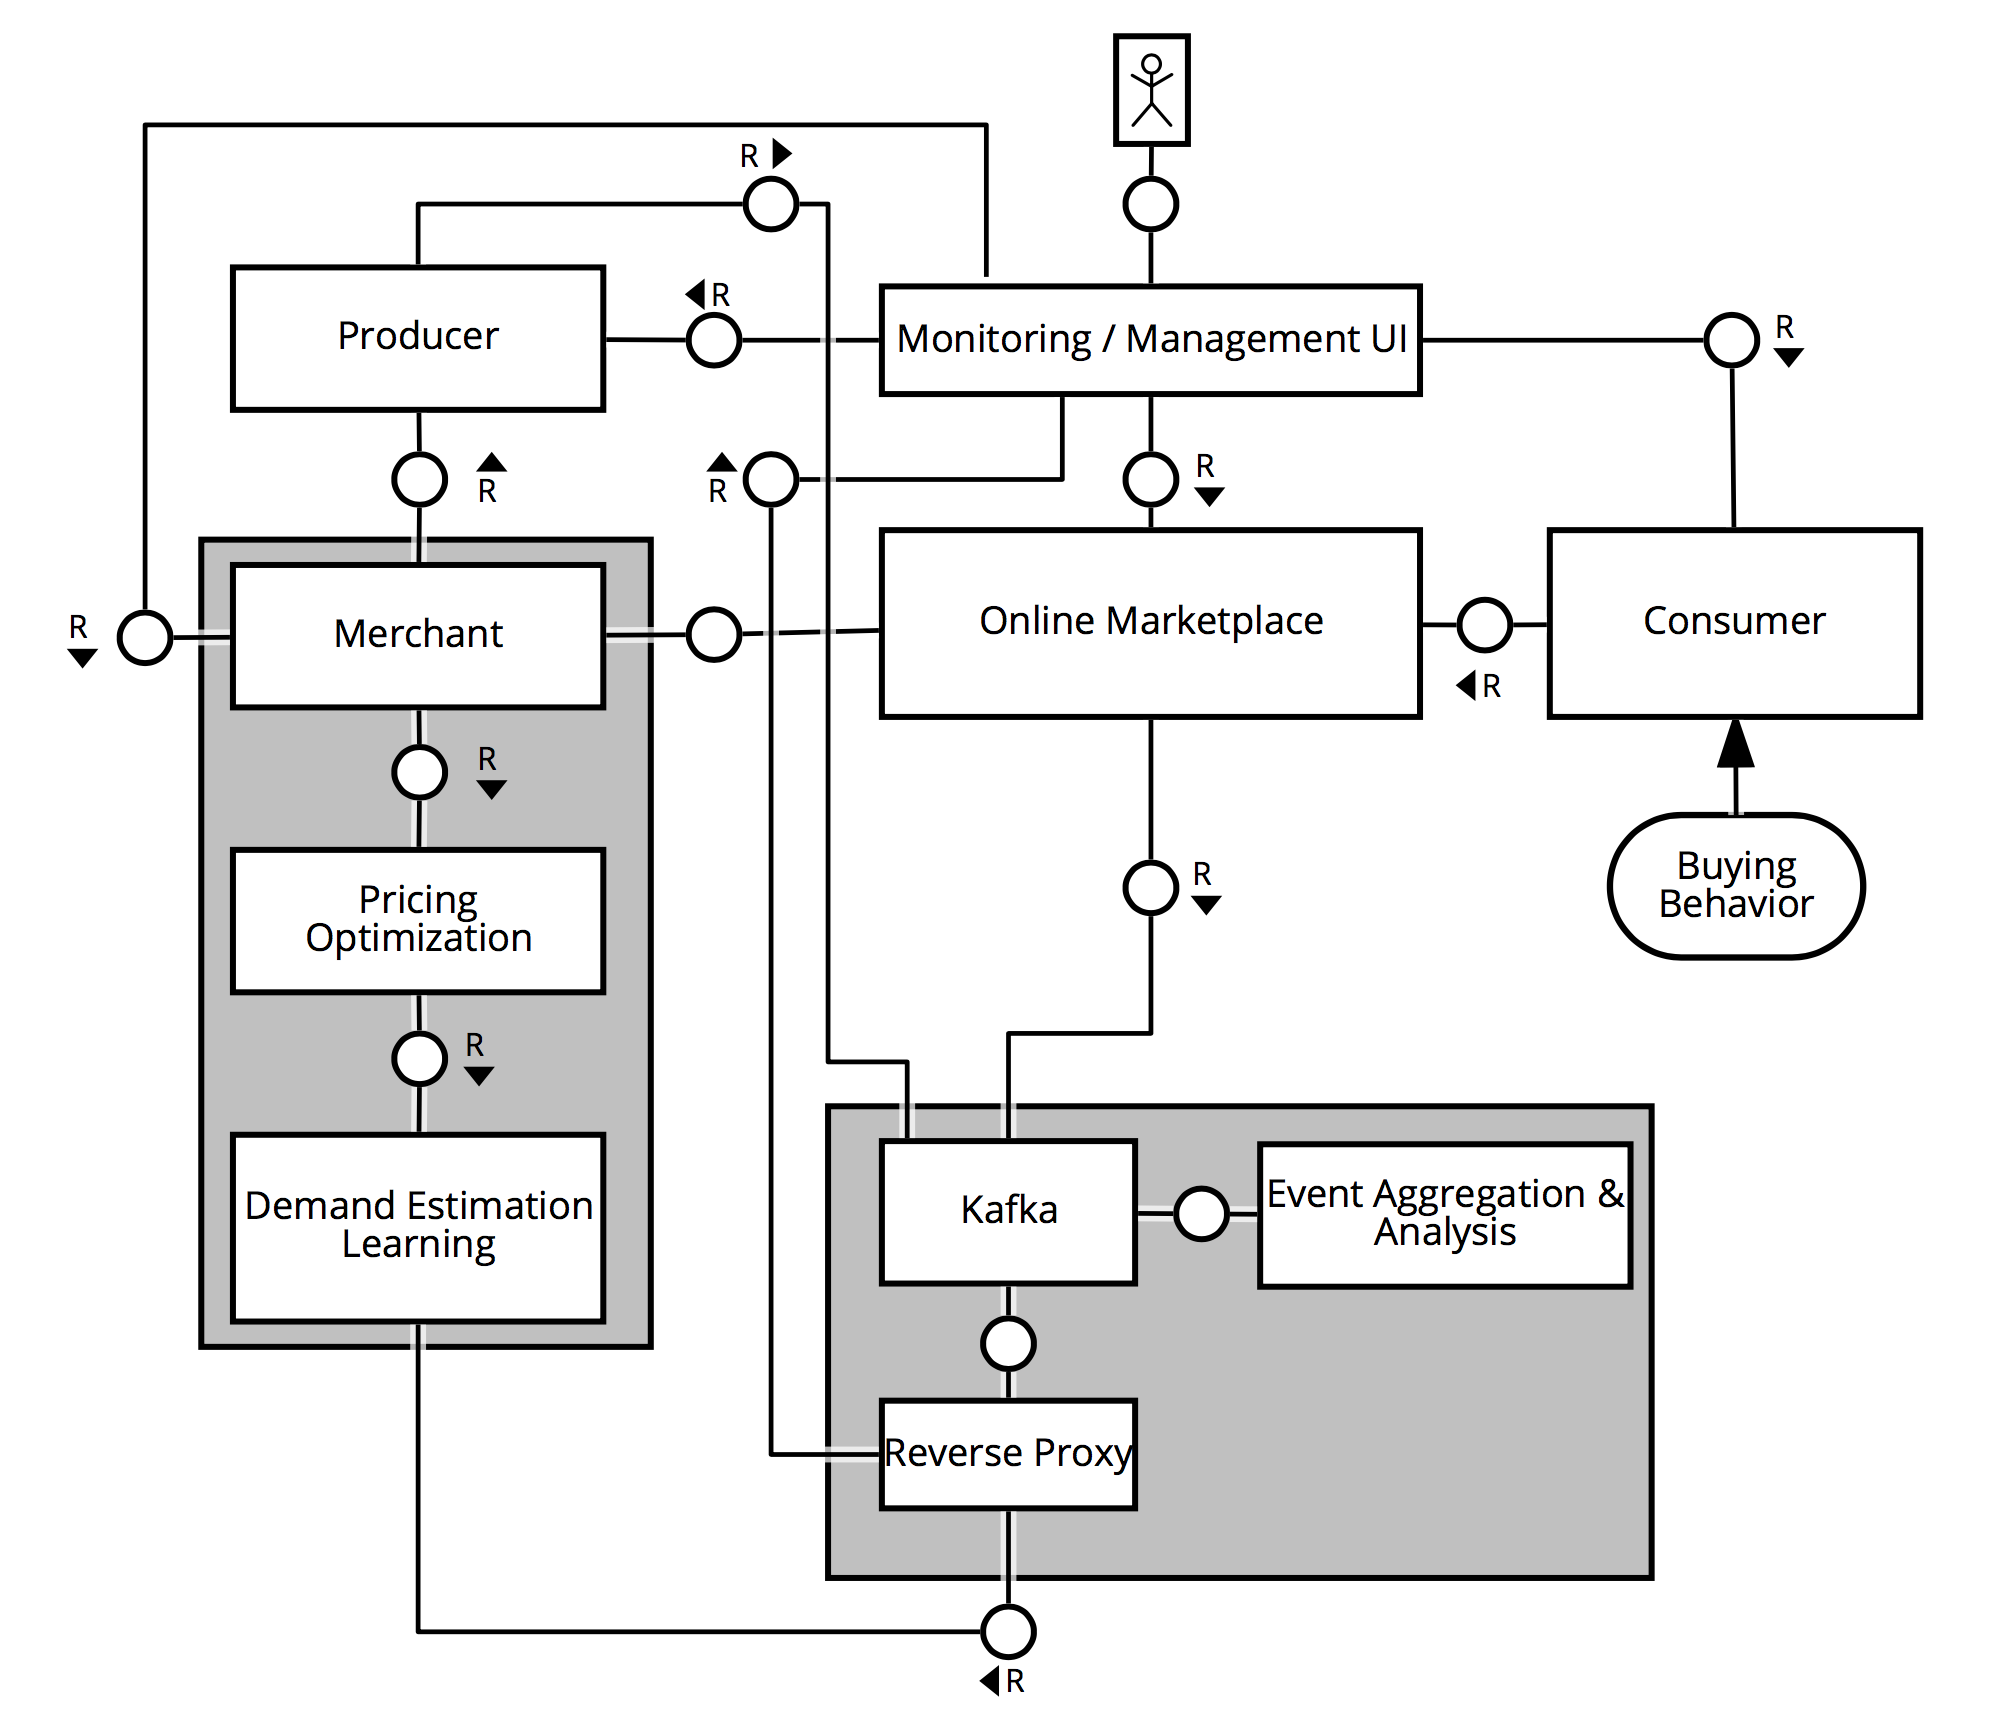
\includegraphics[width=0.5\textwidth]{images/architecture.png}
    \caption{FMC diagram of the Price Wars architecture}
    \label{fig:fmc}
\end{figure}
%